\section{Opis Modelu SI}\label{sec:opis-modelu-si}

Model sztucznej inteligencji został zaprojektowany w celu klasyfikacji zdjęć kości ośmiościennych do jednej z ośmiu klas,
odpowiadających cyfrom od 1 do 8 na każdej ze ścianek.
Do implementacji modelu wykorzystano przede wszystkim moduł TensorFlow~\cite{tensorflow_docs}
oraz wchodzący obecnie w jego skład Keras~\cite{keras_docs},
który umożliwia łatwe tworzenie i trenowanie sieci neuronowych.
%% uselesss :(( \textit{Biblioteka Keras jest wygodnym opakowaniem (wrapperem) dla modeli DL używanych do oszacowań klasyfikacji lub regresji]} [Donald J. Norris, 2020 s. 355 wydanie APN PROMISE SA]

\subsection{Przygotowanie danych}\label{subsec:przygotowanie-danych}

Dane wejściowe zostały podzielone na zestawy treningowy i walidacyjny w proporcji 70:30.
W celu zwiększenia różnorodności danych treningowych zastosowano techniki augmentacji obrazów dostępne w klasie
\texttt{ImageDataGenerator}~\cite{keras_imagedatagenerator}, takie jak:

\begin{itemize}
    \item obrót o losowy kąt w zakresie do 90°,
    \item przesunięcia poziome i pionowe w zakresie $\pm 20\%$ wymiarów obrazu,
    \item transformacje perspektywiczne (ang. \textit{shear}) w zakresie $\pm 10\%$,
    \item losowe przybliżenia lub oddalenia (ang. \textit{zoom}) w zakresie $90\%-110\%$ oryginalnego obrazu.
\end{itemize}

Wszystkie augmentacje przedstawiono na rys.~\ref{fig:5augment}
Dodatkowo, obrazy są normalizowane do zakresu $[0, 1]$, co pozwala na skuteczniejsze działanie sieci neuronowej.

\begin{figure}[h]
    \centering
    \begin{subfigure}[t]{0.32\linewidth}
        \centering
        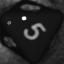
\includegraphics[width=\linewidth]{chapters/04-czytanie/figures/5_preprocessed}
        \caption{Obraz po preprocessingu, bazowy dla augmentacji.}
        \label{fig:5raw}
    \end{subfigure}
    \hfill
    \begin{subfigure}[t]{0.32\linewidth}
        \centering
        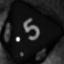
\includegraphics[width=\linewidth]{chapters/04-czytanie/figures/5_rotate}
        \caption{Obraz po obrocie.}
        \label{fig:5rotate}
    \end{subfigure}
    \hfill
    \begin{subfigure}[t]{0.32\linewidth}
        \centering
        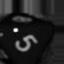
\includegraphics[width=\linewidth]{chapters/04-czytanie/figures/5_shift}
        \caption{Obraz po przesunięciu.}
        \label{fig:5move}
    \end{subfigure}

    \vspace{0.5cm} % Odstęp między wierszami obrazków

    \begin{subfigure}[t]{0.32\linewidth}
        \centering
        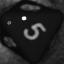
\includegraphics[width=\linewidth]{chapters/04-czytanie/figures/5_shear}
        \caption{Obraz po transformacji perspektywicznej.}
        \label{fig:5shear}
    \end{subfigure}
    \hfill
    \begin{subfigure}[t]{0.32\linewidth}
        \centering
        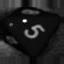
\includegraphics[width=\linewidth]{chapters/04-czytanie/figures/5_zoom}
        \caption{Obraz po powiększeniu.}
        \label{fig:5zoom}
    \end{subfigure}
    \hfill
    \begin{subfigure}[t]{0.32\linewidth}
        \centering
        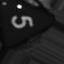
\includegraphics[width=\linewidth]{chapters/04-czytanie/figures/combined_1}
        \caption{Obraz wynikowy.}
        \label{fig:5combined}
    \end{subfigure}

    \caption{Różne składowe augmentacji obrazów uczących}
    \label{fig:5augment}
\end{figure}


W szczególności należy zaznaczyć, że finalnie uniknięto początkowo przeoczonego błędu,
jakim jest tworzenie obrazów lustrzanych w wyżej wymienionych transformacjach, gdyż obrazy lustrzane
sprawiały, że ścianki 2 oraz 5 były znacznie gorzej rozróżniane przez wytrenowany model.
Problem nie był początkowo łatwy do wykrycia, gdyż zdjęcia odbite zarówno w pionowej jak i poziomej osi były poprawne,
a niepoprawne były te odbite tylko względem jednej osi, czego przykład można zaobserwować na rys.~\ref{fig:25confusion}.


\begin{figure}[h]
    \centering
    \begin{subfigure}[t]{0.45\linewidth}
        \centering
        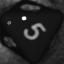
\includegraphics[width=\linewidth]{chapters/04-czytanie/figures/5_preprocessed}
        \caption{Zdjęcie przedstawiające 5}
        \label{fig:5_confusion}
    \end{subfigure}
    \hfill
    \begin{subfigure}[t]{0.45\linewidth}
        \centering
        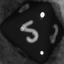
\includegraphics[width=\linewidth]{chapters/04-czytanie/figures/2_mirror}
        \caption{Zdjęcie przedstawiające 2, odbite lustrzanie}
        \label{fig:2_confusion}
    \end{subfigure}
    \caption{Wizualne przedstawienie problemu dot. odbicia lustrzanego}
    \label{fig:25confusion}
\end{figure}
